% http://www.latexstudio.net/archives/2234.html
% 函数绘图实例
% 如何画出 x^(2/3) + y^(2/3) = a^(2/3) 的函数图像?其中 a=2。


% 原生 TikZ 代码实现代码:
% 注意事项:
% line cap 有三种,分别是:round,butt,rect,区别参看:line cap
% line join 有三种,分别是:miter,bevel,round,区别参看:line join
% 这里用到了 abs 取 x 的绝对值,如果不使用将缺少一半,原因不太清楚。
% samples 取样点奇数与偶数有点小差别,视情况选择奇数或者偶数,在这里选择奇数 samples=201。
\documentclass[tikz,border=3pt]{standalone}

\usepackage{mathpazo}
\newcommand{\num}{2.2}
 % define the style elegant
\tikzset{elegant/.style={domain=-2:2,thick,samples=201,magenta,line cap=rect,line join=bevel}}


\begin{document}

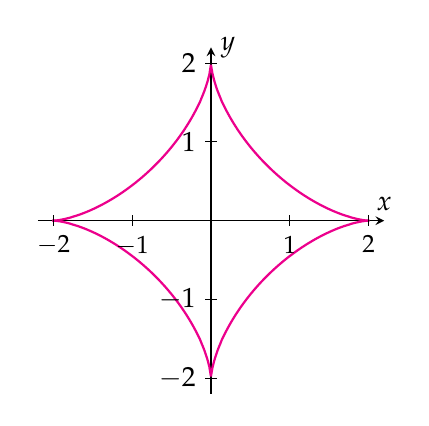
\begin{tikzpicture}[>=stealth]
    % draw the axis
    \draw[->] (-\num,0) -- (\num,0) node[above] {$x$};
    \draw[->] (0,-\num) -- (0,\num) node[right] {$y$};
    % draw the part above of x axis
    \draw[elegant] plot (\x,{(2^(2/3) - (abs(\x))^(2/3) )^(3/2)});
    % draw the part below of x axis
    \draw[elegant] plot (\x,{-(2^(2/3) - (abs(\x))^(2/3) )^(3/2)});
    \foreach \x/\xtext in {-2/-2, -1/-1, 1/1, 2/2}
    \draw[shift={(\x,0)}] (0pt,2pt) -- (0pt,-2pt) node[below] {\small $\xtext$};
     \foreach \y/\ytext in {-2/-2, -1/-1, 1/1, 2/2}
    \draw[shift={(0,\y)}] (2pt,0pt) -- (-2pt,0pt) node[left] {$\ytext$};
\end{tikzpicture}

\end{document}